\documentclass{beamer}
\usetheme{Madrid}
\usepackage{multicol}
\definecolor{ReedRed}{RGB}{167, 14, 22} %Reed Red (primary)
\usecolortheme[named=ReedRed]{structure}
\useoutertheme{miniframes}
\useinnertheme{circles}
\usepackage{soul}

\usepackage{listings}


\usepackage{multicol}
\usepackage{tikz}
\usetikzlibrary{snakes}
\usepackage{rotating}

\usepackage[style=apa,backend=biber,citestyle=numeric]{biblatex}
\addbibresource{../refs.bib}

\title{Bayesian Neural Networks}
\author{
	Ava, Conor, \& Taylor
}
\logo{
	
\includegraphics[width=1cm]{../Images/reed-logo.png}
}
\institute{Reed College}
\setbeamertemplate{navigation symbols}{} % Remove nav bar

\begin{document}
	\section{Intro}
	
\begin{frame}[plain]
    \maketitle
\end{frame}



\begin{frame}{A Brief History}
	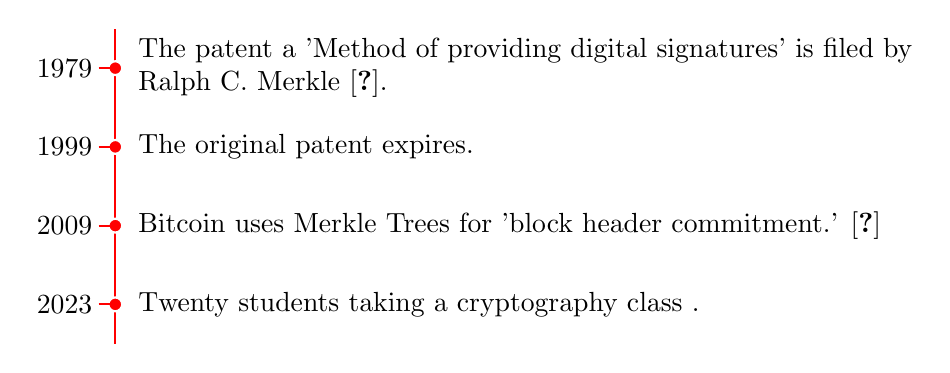
\begin{tikzpicture}[scale=0.5,every node/.style={outer sep=5pt}]
		%Notation: {year, the title of the event}
		%NOTE! Everyting is zero-based
		\def\ourInfo{{
				{"1979"," The patent a 'Method of providing digital signatures' is filed by \\ Ralph C. Merkle  \cite{merkle-patent}."},
				{"1999","The  original patent expires."},
				{"2009","Bitcoin uses Merkle Trees for 'block header commitment.' \cite{friedenbach_alm_2017}"},			
				{"2023","Twenty students taking a cryptography class ."},
		}}
		\pgfmathsetmacro{\length}{3}% Zero based.
		
		% Loop through the array containing all events.
		\foreach \i in {0, ..., \length}{
			\pgfmathsetmacro{\year}{\ourInfo[\i][0]}% Get the left cell (year)
			\pgfmathsetmacro{\eventName}{\ourInfo[\i][1]}% Get the right cell (event name)
			\draw[thick,red] (0,-2*\i-2)--(0,-2*\i);% Draw vertical line
			\ifnum \i=0 % Should be in red text
			\draw(0,-2*\i-1) node[black, right, align = left]{\eventName};% Display the event name
			\draw(0,-2*\i-1) node[black, left] {\year};
			\else % Should be in black text
			\draw(0,-2*\i-1) node[right, black]{\eventName};% Display the event name
			\draw(0,-2*\i-1) node[left] {\year};% Display the year
			\fi
		}
		% Draw the bullet with the dash
		\foreach \i in {0, ..., \length}{
			\filldraw[draw = white, fill = red,thick] (0,-2*\i-1) circle (5pt);
			\draw[thick,red] (-12pt,-2*\i-1)--(0,-2*\i-1);
		}
	\end{tikzpicture}
\end{frame}

\begin{frame}{Applications}
	\begin{multicols}{2}
		\begin{figure}
			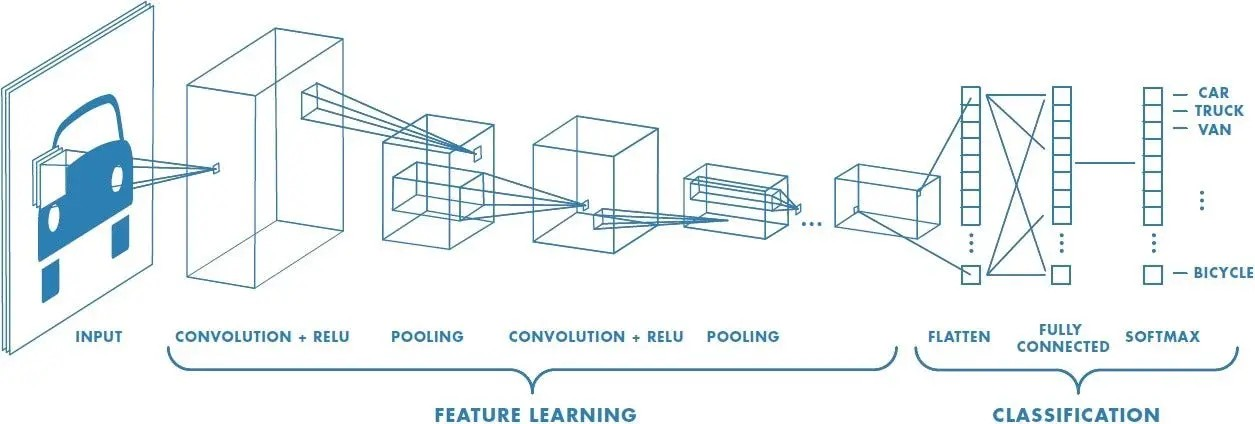
\includegraphics[width=.45\textwidth]{../Images/big-pic-cnn.jpg}
			\caption{Relevant XKCD needed... }
		\end{figure}
		
		\columnbreak
		
		\null \vfill
		
		What are .
		%Shrinking public keys. \cite{boneh2020graduate}
		
		\vfill \null
	\end{multicols}
\end{frame}

\section{Neural Networks}

\begin{frame}{Neural Networks (NN)}
	% A convolutional neural network has the same structure as a regular neural network
	% Except we slide over the image and take k
	\begin{figure}
	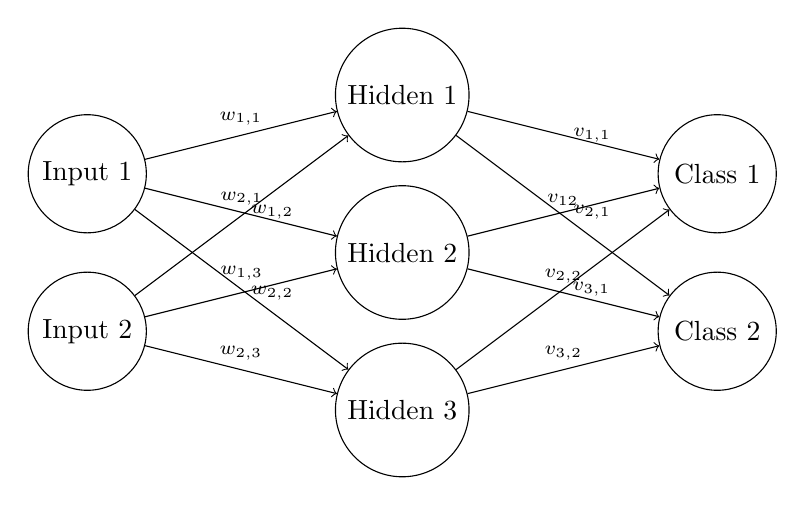
\begin{tikzpicture}
		% Define node styles
		\tikzstyle{neuron} = [circle, draw, minimum size=1.5cm];
		\tikzstyle{weight} = [font=\scriptsize];
		
		% Input layer (2 neurons)
		\node[neuron] (input1) at (-2,1) {Input 1};
		\node[neuron] (input2) at (-2,-1) {Input 2};
		
		% Hidden layer (3 neurons)
		\node[neuron] (hidden1) at (2,2) {Hidden 1};
		\node[neuron] (hidden2) at (2,0) {Hidden 2};
		\node[neuron] (hidden3) at (2,-2) {Hidden 3};
		
		% Output layer (2 neurons for classification)
		\node[neuron] (output1) at (6,1) {Class 1};
		\node[neuron] (output2) at (6,-1) {Class 2};
		
		% Connections with weights
		\draw[->] (input1) -- node[weight, above] {$w_{1,1}$} (hidden1);
		\draw[->] (input2) -- node[weight, above] {$w_{2,1}$} (hidden1);
		\draw[->] (input1) -- node[weight, right] {$w_{1,2}$} (hidden2);
		\draw[->] (input2) -- node[weight, right] {$w_{2,2}$} (hidden2);
		\draw[->] (input1) -- node[weight, above] {$w_{1,3}$} (hidden3);
		\draw[->] (input2) -- node[weight, above] {$w_{2,3}$} (hidden3);
		\draw[->] (hidden1) -- node[weight, right] {$v_{1,1}$} (output1);
		\draw[->] (hidden2) -- node[weight, right] {$v_{2,1}$} (output1);
		\draw[->] (hidden3) -- node[weight, right] {$v_{3,1}$} (output1);
		\draw[->] (hidden1) -- node[weight, above] {$v_{12}$} (output2);
		\draw[->] (hidden2) -- node[weight, above] {$v_{2,2}$} (output2);
		\draw[->] (hidden3) -- node[weight, above] {$v_{3,2}$} (output2);
	\end{tikzpicture}
		\caption{Example neural network}
	\end{figure}
\end{frame}

\begin{frame}{Issues with Neural Networks}
	\begin{multicols}{2}
		\begin{figure}
			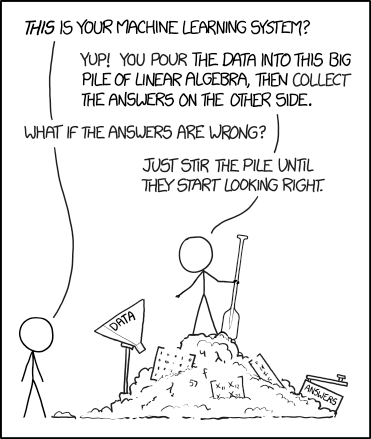
\includegraphics[width=.4\textwidth]{../Images/xkcd_machine_learning.png}
			\caption{XKCD: "\textit{Machine Learning}" \cite{xkcd-ml}}
		\end{figure}
		
		\columnbreak
		
		\null \vfill
		\begin{itemize}
			\item Stir data and pray
			\item 
		\end{itemize}
		\vfill \null
	\end{multicols}
\end{frame}

\begin{frame}{Convolutional Neural Networks (CNN)}
	% A convolutional neural network has the same structure as a regular neural network
	% Except we slide over the image and take k
	\begin{figure}
		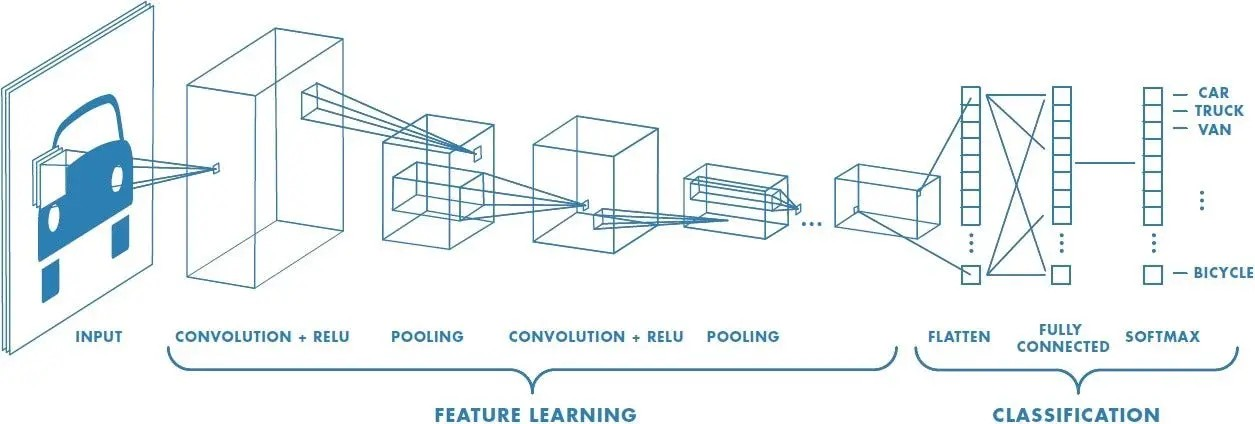
\includegraphics[width=.8\textwidth]{../Images/big-pic-cnn.jpg}
		\caption{CNN pipeline \cite{eli5CNN}}
	\end{figure}
\end{frame}

\begin{frame}{Why we use CNNs}
	\begin{multicols}{2}
		\begin{figure}
			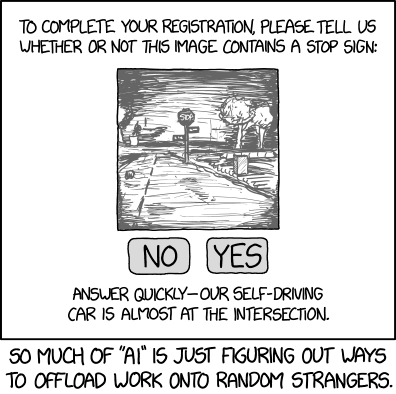
\includegraphics[width=.45\textwidth]{../Images/xkcd_self_driving.png}
			\caption{XKCD: "\textit{Self Driving}" \cite{xkcd-self-driving}}
		\end{figure}
		
		\columnbreak
		
		\null \vfill
		\begin{itemize}
			\item They are more efficient for image based tasks
			\item Channels...
		\end{itemize}
		\vfill \null
	\end{multicols}
\end{frame}

\section{Bayesian Neural Networks}

\begin{frame}{Bayesian Neural Network}
	% The relationship between BNN and CNNs is the same as NNs and CNNs
	\begin{figure}
		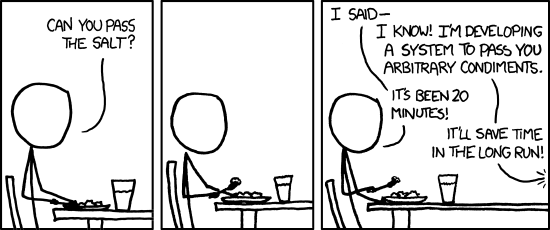
\includegraphics[width=.75\textwidth]{../Images/the_general_problem.png}
		\caption{ XKCD: "\textit{The General Problem}" \cite{xkcd-general-problem}}
	\end{figure}
	The relationship between BNNs and BCNNs is the same as NNs and CNNs.
\end{frame}


\begin{frame}{Difference between BNNs and BCNNs}
	% The relationship between BNN and CNNs is the same as NNs and CNNs
	\begin{figure}
		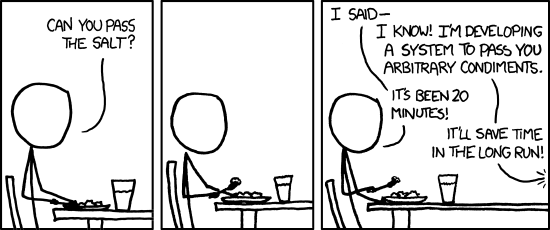
\includegraphics[width=.75\textwidth]{../Images/the_general_problem.png}
		\caption{ XKCD: "\textit{The General Problem}" \cite{xkcd-general-problem}}
	\end{figure}
		The relationship between BNNs and BCNNs is the same as NNs and CNNs.
\end{frame}


\section{Simulation}

\begin{frame}{CIFAR-10}
	% A convolutional neural network has the same structure as a regular neural network
	% Except we slide over the image and take k
	\begin{figure}
		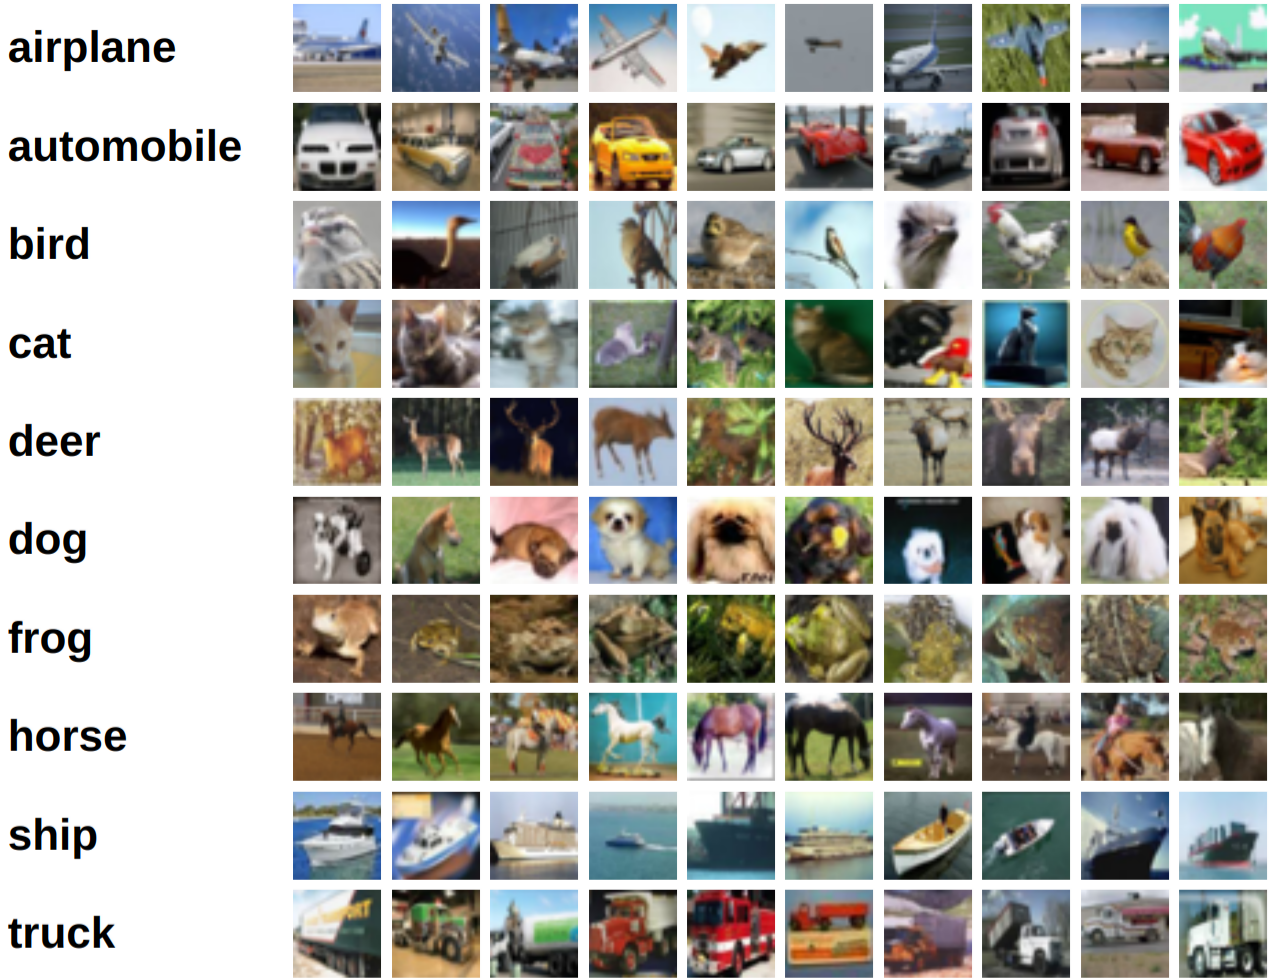
\includegraphics[width=.65\textwidth]{../Images/cifar-10.png}
		\caption{Example CIFAR-10 images \cite{cifar10}}
	\end{figure}
\end{frame}

\begin{frame}{Hyperparameters}
	% Replace cell text later
	\centering
	\begin{tabular}{|c||p{3cm}|p{3cm}|} % Adjust p{width} as needed
		\hline
		\textbf{Hyperparameter} & \textbf{CNN} & \textbf{BCNN} \\ [0.5ex] 
		\hline\hline
		Epochs & 500 & 500\\
		\hline
		Learning Rate & ....  & May be higher (0.01 - 0.1) due to simpler structure  \\
		\hline
		Regularization & L1/L2 weight decay or Dropout common to prevent overfitting & Can benefit from Dropout, but weight decay might be less crucial \\
		\hline
		Optimizer & Adamw  & Adamw  \\
		\hline
	\end{tabular}
\end{frame}

\begin{frame}{Results}
	% Image Later
	\begin{figure}
		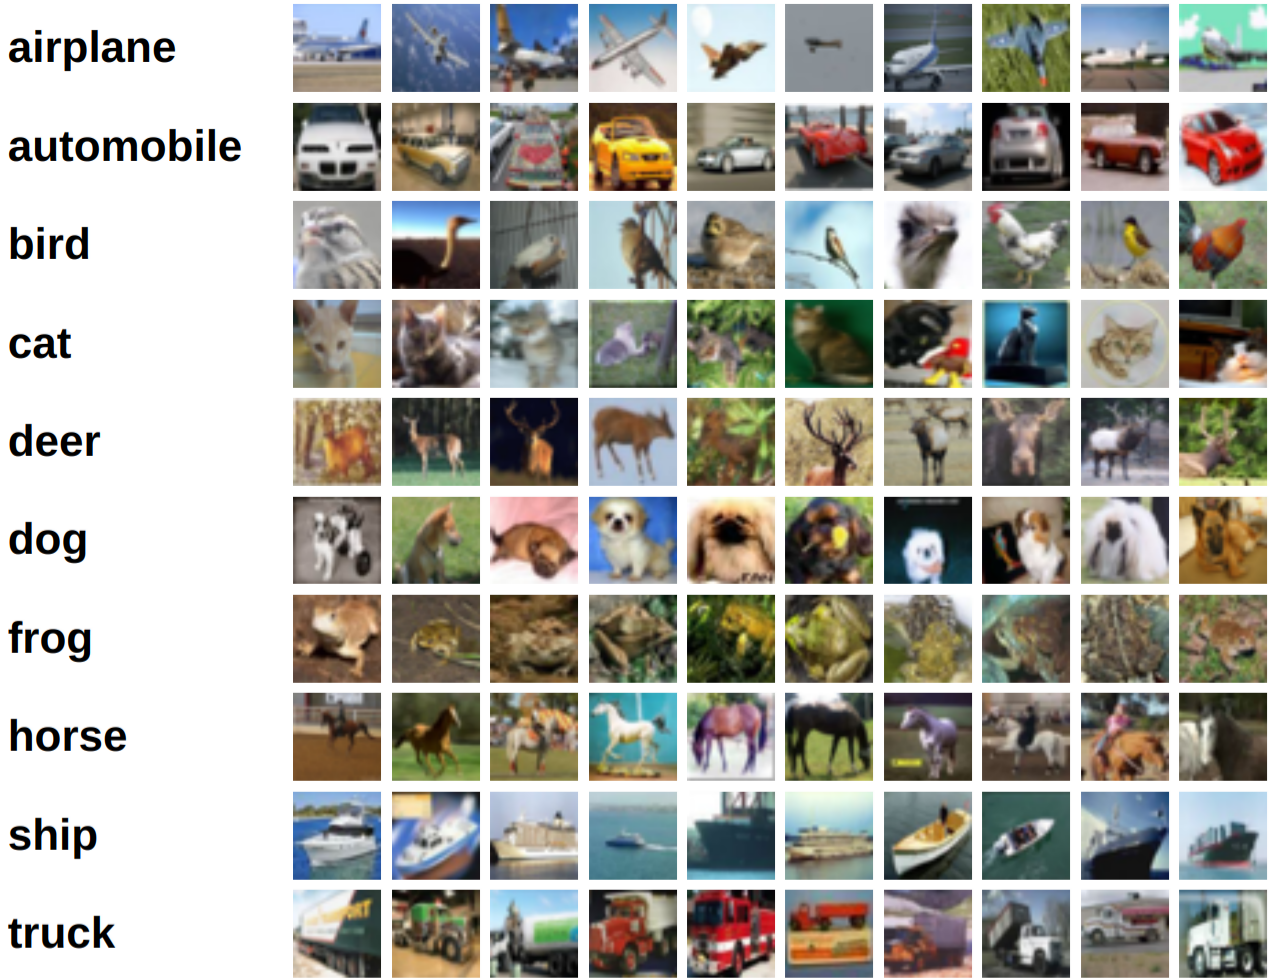
\includegraphics[width=.65\textwidth]{../Images/cifar-10.png}
		\caption{Example CIFAR-10 images \cite{cifar10}}
	\end{figure}
\end{frame}

\begin{frame}{Confusion Matrix}
	% Image Later
	\begin{figure}
		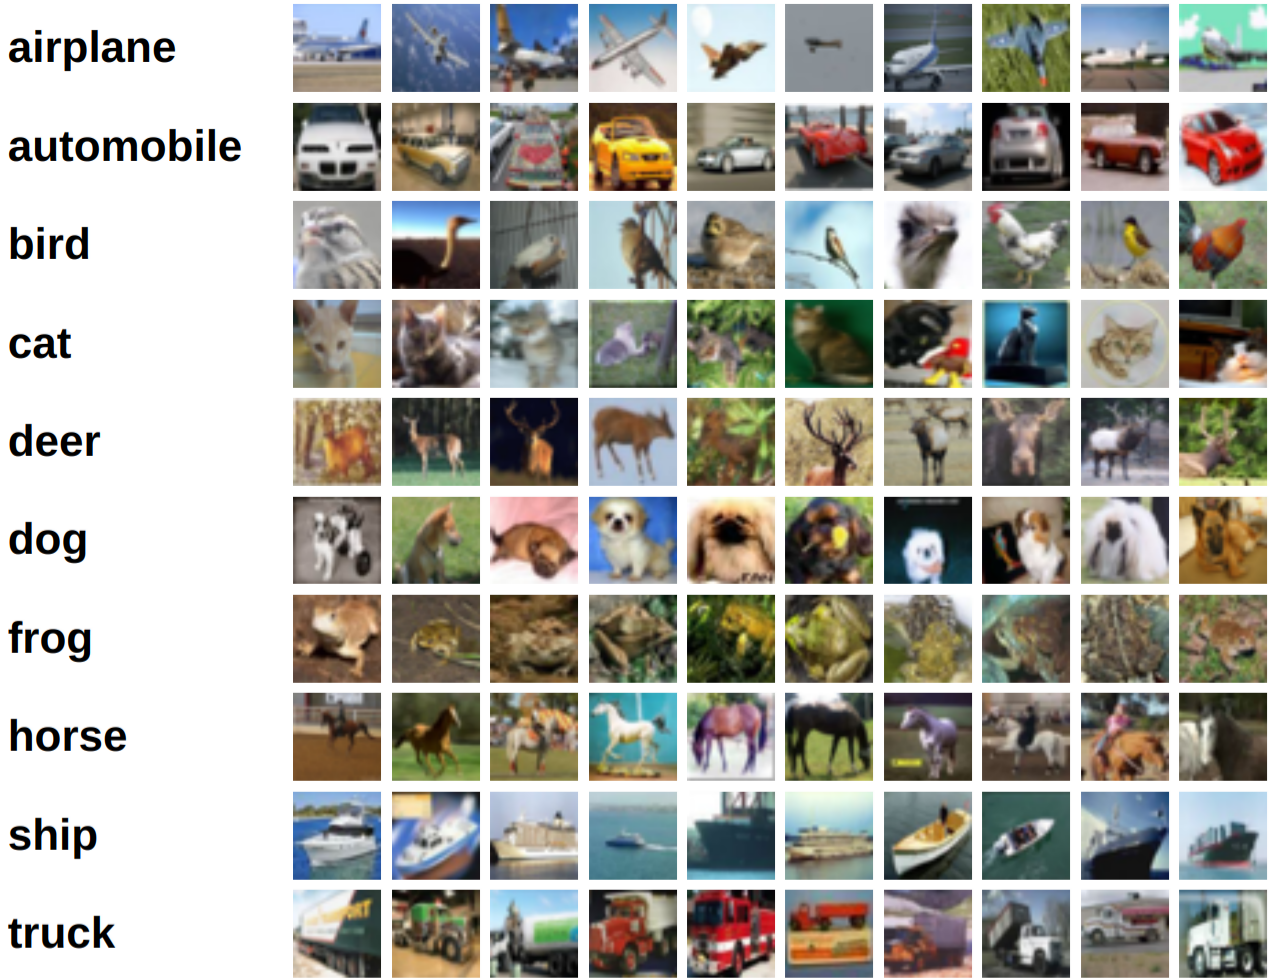
\includegraphics[width=.65\textwidth]{../Images/cifar-10.png}
		\caption{Example CIFAR-10 images \cite{cifar10}}
	\end{figure}
\end{frame}


\begin{frame}[allowframebreaks]{References}
\printbibliography
\end{frame}

\end{document}
